\chapter{Introduction}
\label{chap:Introduction}

Augmented reality (AR) systems combine standard video inputs with computer-generated objects and
usually provide real-time interaction for the users. 
In general, an augmented reality system can be defined with the following properties \cite{azuma01,milg94} :
\begin{itemize}
\item Combination of real and virtual environment
\item Registration (alignment) of real and virtual objects
\item Real-time interaction
\end{itemize}
This concept was pioneered in the 1960s by an American computer scientist named Ivan Sutherland
who created the first head-mounted augmented reality
system with the help of one of his students \cite{azuma01}.

Combining virtual objects and annotations with real
world scenes has proved to be an effective way of conveying information about the surrounding environment to
the user and can be useful in many applications such as gaming, medical surgeries, tourism, and other entertaining, informative or instructional tasks.

Many mobile augmented reality systems have been built over the past decades, from the Touring Machine in 1997 by Feiner et al. \cite{fei97} 
to Google AR glasses which was announced in 2013 \cite{google}; however, most of these prototypes have remained experimental
due to certain difficulties and constraints of using them in practical applications \cite{dras96,liv05}. To name two of the most important constraints
we can refer to:
\begin{enumerate}
\item Human factors in augmented reality 
\item High demand of computational resources in order to provide a real-time interaction between the user and the system
\end{enumerate}

%\section{Obtaining Depth Cues in AR Systems}
\section{Image Registration in Augmented Reality}
AR systems overlay 2D or 3D virtual objects on real scenes. Therefore, depending on the application, certain accuracy is required for 
registration of the virtual and real objects in the scene, for which certain knowledge of the location of the user and different objects 
is essential \cite{azuma01,milg94}.
In an AR system, different techniques can be used to 
obtain the user's location and the position of other objects in the environment. In many AR systems, fiducial markers are used
in the environment with computer vision tracking methods to find the actual position of the objects within the scene. This method, however, is 
more useful in prepared, indoor AR environments. Tracking sensors such as gyroscope and accelerometer along with video sensors can 
also be used as complementary techniques to provide information on the user's position and viewing orientation \cite{azuma01}. 
%however, they usually rely on known features in the surrounding environment.
However, for unprepared, outdoor environments, especially in mobile AR applications, it is not practical to use markers in various locations 
in the scene and, therefore, a markerless technique, such as obtaining a dense depth map of the surrounding environment,
must be considered as an alternative to find the position of the objects in the scene.
To obtain the depth of the 
surrounding environment several depth sensing technologies can be used such as 3D laser scanner, depth cameras or regular cameras. However, in order to have a mobile AR
system that is easy to carry around, the weight of the whole system will be more of a concern, hence, 
3D laser scanners and depth cameras are not proper choices for such systems.
Depth cameras, such as Kinect, or DS325 have a strong limitation in the viewing range; Kinect, 0.8m to 4m \cite{mkinect}; and DS325, 0.15m to 1m \cite{skinetic}. 
On the other hand, 3D laser scanners can
generate very accurate depth maps; however, they are normally expensive and their price ranges from \$3,000 to \$300,000 or more, 
depending on their accuracy and range.
Therefore, among all these technologies, using several 
cameras to generate a depth map of the surrounding environment seems to be a more practical approach for outdoor mobile augmented reality systems. {\newline}
However, using several cameras to get the depth map of the scene requires certain conditions to be met, geometrically and computationally. Many researchers have already looked into
this particular problem, i.e, finding the 3D position of the points in the scene from two or multiple views using regular cameras \cite{sze11}. Attempts of these researchers have resulted in
certain techniques in computer vision to find the depth of different points in an environment using one or more stereo pairs taken from slightly different points of view of the same scene.
These techniques are known as {\it Stereo Correspondence} or {\it Stereo Matching} in computer vision \cite{sze11}. Stereo matching has been one of the most studied subjects in computer vision for 
many years now and there are many solutions proposed by researchers to address this problem using different techniques; however, finding the corresponding pixels in stereo pairs with certain level of 
accuracy and in real-time for practical applications still remains a challenging task. {\newline}

% Motivation - Objective - Contributions %
\section {Motivation}

Due to the emergence of different techniques to solve the problem of stereo correspondence, having an evaluation scheme to assess 
these solutions is essential. Over the past few years, different evaluation schemes have been proposed 
by researchers in the field to provide a testbed for assessment of the solutions based on specific criteria.
For instance, the Middlebury Stereo \cite{mideval} and the Kitti Stereo benchmarks \cite{kitti}
are two of the most popular and widely used evaluation systems through which a solution can be evaluated and compared 
to others. 
However, both of these models take a general approach towards evaluating the methods, that is, they 
have not been designed with an eye to the particular target application. In other words, 
they mainly focus on the fundamental aspects of designing a stereo algorithm as a solution per se to generally
find the \textit{best matches} of corresponding pixels in stereo pairs. 

In this study, we take steps towards an evaluation design which is based on the potential 
applications of stereo vision methods.
This enables us to better define and adjust the criteria for \textit{efficiency} and 
\textit{the best correspondence matches} while doing the evaluation.
Since AR has attracted more attention in the past few years, 
the evaluation scheme proposed in this study is designed based on outdoor AR applications which take advantage of
stereo vision techniques to obtain a depth map of the surrounding environment. This map will then be used to
integrate virtual objects in the scene that respect the occlusion property and the depth of the real objects in the scene. 

In other words, our motivation in this research is to study the possibility of combining stereo vision approaches with 
AR systems considering the most important constraints that AR systems
normally encounter in outdoor environments. 
In fact, our fundamental research question is: \newline

\begin{quote}
\textbf{``Can the combination of stereo matching techniques with augmented reality meet the requirements of an AR system in outdoor 
environments?''} \newline
\end{quote}
\noindent
To provide an informed answer to the previous question, we believe that the following more fundamental questions need to be answered first:  
\begin{quote}
\textbf {``How does the human visual system (HVS) perceive depth?''}\newline
\textbf {``What is the standard angular disparity for the human visual system and how would it affect an AR system?''} \newline
\textbf {``How can we evaluate stereo vision in an augmented reality framework and what are the important factors we need to consider for 
	this type of evaluation?''} \newline
\textbf {``In a combination of augmented reality with stereo vision, what is considered an \textbf{\textit {accurate}} depth result?''} \newline
\textbf {``How can a three dimensional model be built from stereo images using computer vision techniques?''}\newline
\textbf {``What are the requirements to maintain an interactive augmented reality application for the user?''} \newline
\end{quote}

To answer these questions, we have designed and implemented a testbed for evaluation of
the stereo matching solutions based on specific criteria which will be thoroughly described in the following chapters.

As a starting point for our AR system, the depth map generated from two or multiple camera views
will be used as the depth source to determine the position of the objects in the scene when
overlaying virtual objects at different locations and depth levels in the real environment. 
For our research, we decided to narrow down our study to the effect of using stereo vision techniques
on two of the most important constraints of an AR system mentioned earlier in this chapter: 
{\it human factors} and {\it real-time interaction}. {\newline}
Human perception of depth can vary depending on the environment and under different circumstances. Many studies have focused on the evaluation of human perception of depth within different frameworks
and in different applications, such as virtual reality and augmented reality, which have recently 
attracted more attention \cite{wann95,dras96,liv05,jer05,swa07,kru10}.
These studies show that the viewer perception of depth
is inversely proportional to his/her distance from the object \cite{kru10,swa07,jer05,liv05}. For instance, in \cite{swa07} some experiments are designed to study and evaluate human
perception of distance, which is the absolute depth of the objects from the observer, for an outdoor augmented reality application in urban settings. 
However, in this research we are more interested in the human perception of relative depth in stereo vision, which is the ability to perceive and distinguish 
the depth of different objects relative to each other. 
In binocular vision, the minimum depth difference between two points 
that can be detected in the visual system is known as {\it Stereoscopic Acuity} or {\it Stereoacuity} \cite{pfa2000}. More detail about
this metric will be provided in the following chapters.
We have investigated the standard stereoacuity in the human visual system and applied it to our evaluation in order to obtain the smallest detectable depth of 
objects in human binocular vision based on their distance from the observer.

Providing real-time interaction in an AR system for the user requires the processing time and update rate of the whole system to keep up ideally with the standard video frame rate, 
between 24fps and 
30fps, or higher. 
However, studies show that in practice to build a reasonable interactive augmented world the processing rate should not be less than half of the video frame rate \cite{hertz00}. 
There are different approaches to speed up a system: 
\begin{enumerate}
\item Using more advanced technology and hardware
\item Achieving a more sophisticated and efficient software design
\end{enumerate}
However, having access to advanced technology and hardware is not always feasible and even the most advanced 
technologies have some limitation in their memory space and computational capability
which may not meet the requirement for some real-time applications. 
Therefore, we have decided to focus more on the second approach while designing our evaluation system which also looks into one of the
key properties of an AR system mentioned earlier, that is, the real-time user interaction.

One of the most important features that makes our evaluation unique and different from the others is that we have 
designed the evaluation process of the stereo matching solutions with an eye to augmented 
reality applications in outdoor environments.
In order to address the speed factor, we evaluate the results based on the requirements of providing an interactive AR system for the user.
In addition, to address the constraint of computational resource, we have integrated a module in our design that 
focus on the evaluation of particular regions in the scene rather than 
the whole image. 
It is known that distinctive features such as {\it edges}, either in RGB or depth images from a scene, 
play an important role in many computer vision applications, such as object detection and 
tracking, determination of a set of reliable correspondences to build a 
3D model that helps with better perception of object locations in 3D space \cite{mart01,sze11}.
Therefore, in an augmented reality application, wrong depth results, especially in those regions, 
which will lead to erroneous registration of virtual and real objects, 
can be perceived easier by the human visual system. This can lead to poor performance of the system and possibly faulty interaction between 
the user and the augmented world.
Figure \ref{fig:ARreg} shows an accurate and faulty registration of objects (the lamp, the head and the synthetic triangle) in a 3D environment that results from an accurate and 
wrong disparity map in a specific area of depth discontinuity.

\begin{figure}[H]
\centering
\subcaptionbox{Accurate registration of objects}
[.5\linewidth]{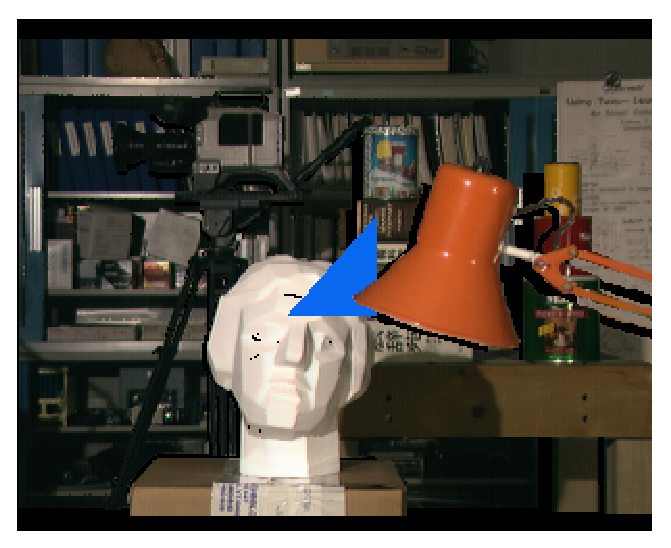
\includegraphics[scale=0.7]{tsukuba}}%
\subcaptionbox{Erroneous registration of objects}
[.5\linewidth]{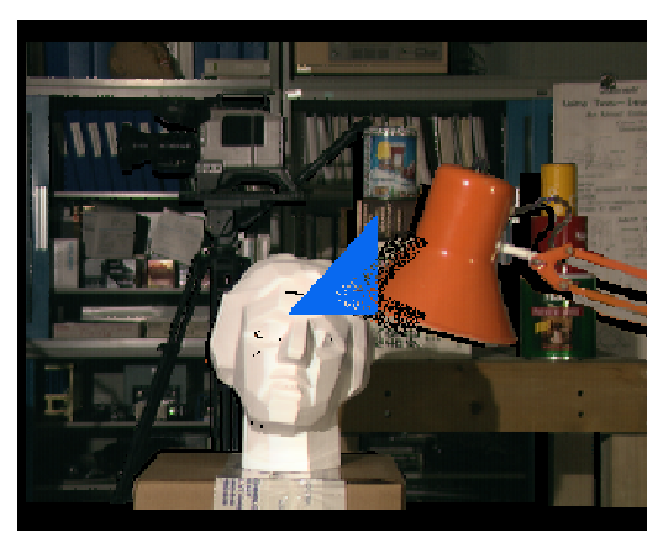
\includegraphics[scale=0.7]{tsukubadist}}%
\caption{Integration of objects in a 3D environment}
\label{fig:ARreg}
\end{figure}

Therefore, we focus the evaluation in our model
on the depth edges in the scene and their surrounding regions \cite{liv05,kru10}.
Our hypothesis is that salient edges caused by depth discontinuities, which can also represent the object boundaries and occlusion, and their surroundings
are one of the most important depth cues for the observer 
to perceive the depth of different objects in the scene \cite{sze11}. 
Furthermore, the regions of depth discontinuity and occlusion are known as two of the most challenging parts in the image
for the stereo correspondence algorithms \cite{sch02}.
Finding correct depth values in these 
regions can lead to a higher quality combination of the virtual and real objects in the scene, thus providing a more reasonable augmented world 
for the user to interact with.

%%Is this part needed to be in this chapter?%%

\section{Methodology}
To achieve our objectives in this research, we have surveyed some of the existing approaches to solve the problem 
of stereo correspondence and the geometrical principles of the 3D reconstruction from stereo pairs, which will be explained more 
in the next chapters. 
In order to investigate the benefits of our proposed model, we have evaluated two sample stereo matching algorithms in our system. 
These algorithms are:
\begin{enumerate}
\item Semi-global block matching, also known as SGBM, which is a modified version of the semi-global matching by Hirschmuller \cite{hir08}.
\item Our implementation of the solution proposed by Mei et al., ``On building an accurate stereo matching system on graphics hardware'' \cite{mei11}, also known as ADCensus.
\end{enumerate}

SGBM is now integrated in the Open Source Computer Vision Library (OpenCV) \cite{sgbm} and, therefore, we have used this implementation
in our evaluation.
On the other hand, since no implementation of ADCensus is available in the public vision libraries, we have used our own implementation of it 
which we refer to as ADCensusB in this thesis.
Although ADCensus is originally proposed as a GPU-based solution, we have used the CPU implementation of it in our evaluation, as no public GPU-implementation was also available.

SGBM is selected as it has shown to generate acceptable results within 1-2 seconds on the typical test images \cite{hir08}; moreover,
its integration within the OpenCV library has made its usage more common in different applications. 
ADCensus is also currently ranked as one of the best solutions 
for solving the problem of stereo correspondence in terms of general accuracy, regardless of the running time, 
according to the Middlebury evaluation table \cite{mideval}.
In addition, AdCensus does not currently exist in the KITTI evaluation table which motivates us to evaluate our implementation of it
under real world circumstances with outdoor stereo images.

\section{Organization of Thesis}
This report is organized in the following structure.
We discuss a background of the related work and concepts in Chapter 2 where the geometry of stereo vision, 
stereo correspondence problem, and a survey of the stereo solutions will be reviewed. 
Moreover, we will introduce some of the key computer vision techniques employed
during this research work. Chapter 3 introduces some of the most relevant concepts in binocular vision to this study.
In Chapter 4, we will explain our system and its design and components in detail. Chapter 5 discusses the experiments
conducted for the evaluation of the proposed system in the framework of an outdoor AR application.
In Chapter 6, we discuss the shortcomings and benefits of our system based on the results from Chapter 5. 
Consequently, a discussion of the potential aspects for improvement 
and future research will also be provided.

